Compute the response of a series $RL$ circuit to a square wave input as shown in Fig.~\ref{input_wave}, both numerically and analytically. For the numerical approach, use appropriate numerical techniques to solve the differential equation governing the $RL$ circuit's behaviour. For the analytical approach, utilise Fourier Series to derive the response of the circuit. The square wave is characterised by a duty ratio, denoted by the factor $\alpha$. You are free to choose the values of resistance $R$ and inductance $L$ for your analysis.

\begin{figure}[H]
  \centering
  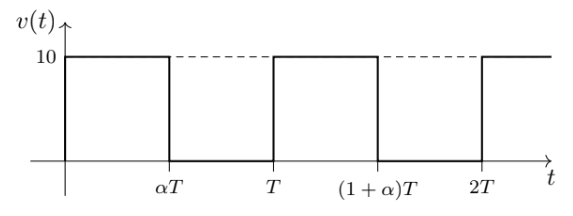
\includegraphics[width=0.5\textwidth]{input_wave.png}
  \caption{Square wave with a duty ratio $\alpha$}
  \label{input_wave}
\end{figure}

Analyse the circuit's behaviour obtained from both numerical and analytical methods. In your analysis, apply the relevant concepts from the course related to circuits and differential equations to explore the response and draw comparisons between the two approaches.
